\section{Workflow and Validation Interfaces}
\label{sec:system}
\subsection{Problem and delivery contract}
A confirmed specification $s$ defines an original objective $f_s(x;d)$ and constraints $c_j(x;d)$ over prepared
data $d$ and binary decisions $x$. After converting the objective to minimization, the compiler builds
\begin{equation}
 E_{\lambda}(x,z;d)=f_s(x;d)+\sum_j\lambda_j P_j(x,z;d),
\end{equation}
where $z$ contains encoding auxiliaries and $P_j$ is the selected constraint penalty. Changing $\lambda$ changes
QUBO energy, so different configurations are ranked by original-constraint feasibility and objective, not raw
energy. Approximate encodings are identified explicitly.

Inputs are classified as public facts, user settings or private data. Public fields require source records;
settings are confirmed rather than searched for. Private inputs must be provided or explicitly marked as mock.
The output includes the specification, prepared data and provenance, model, solution, figure and assumptions.
Delivery states whether the solution came from annealing or a conventional baseline, and distinguishes usable,
limited-quality and unavailable outputs.

\begin{figure*}[t]
\centering
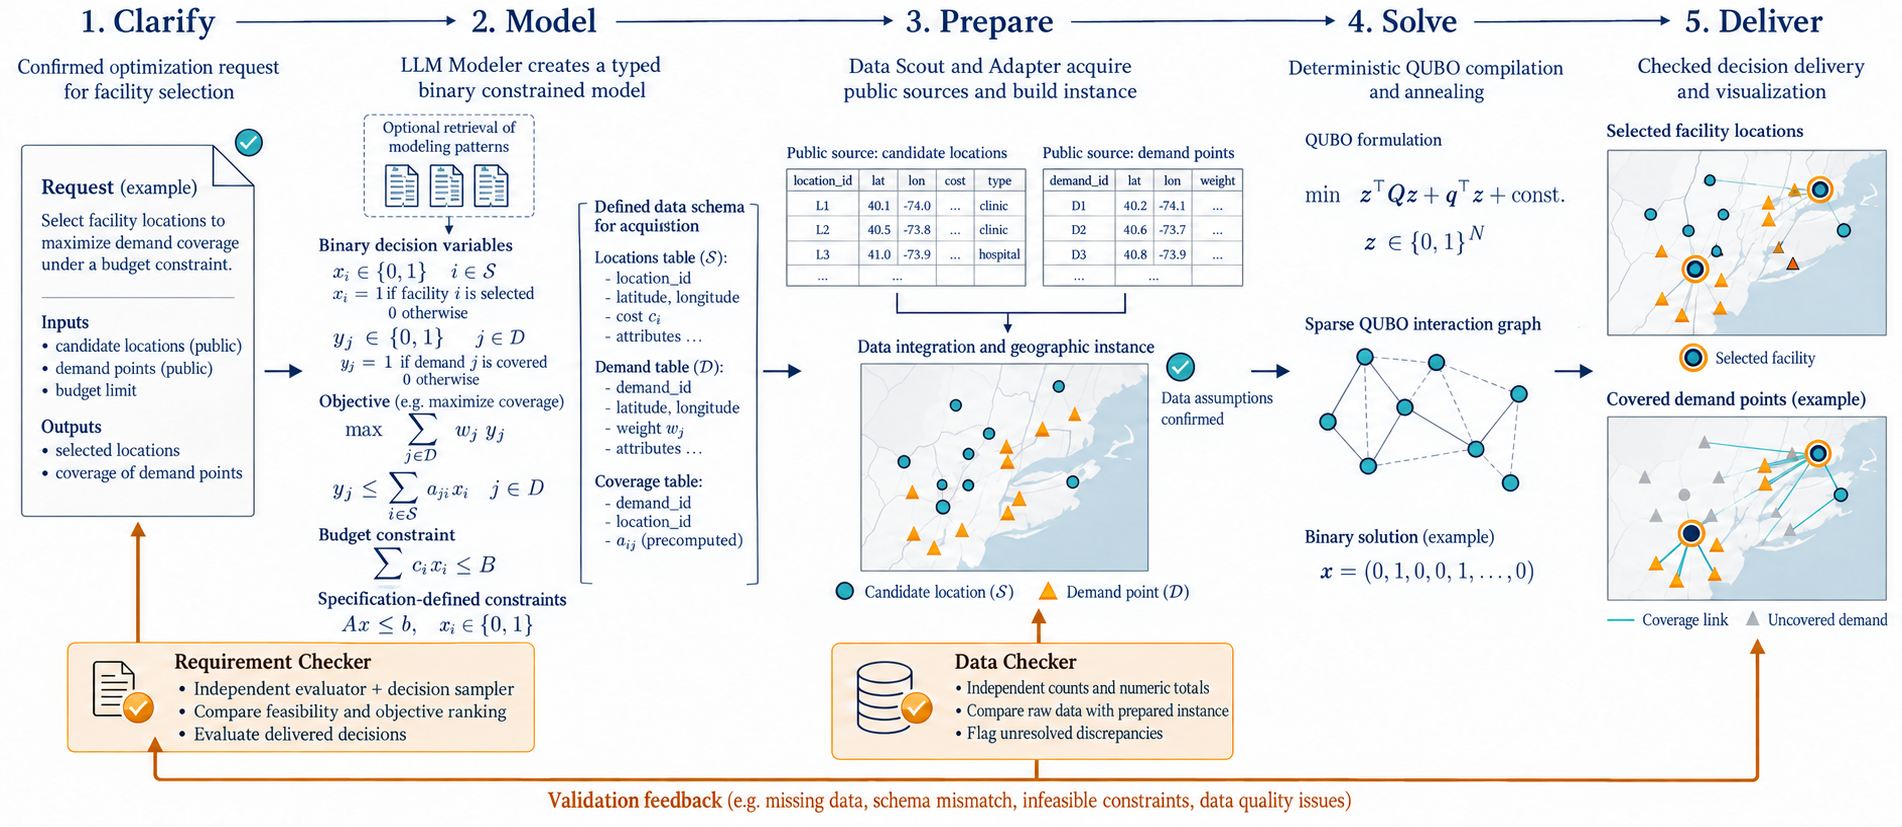
\includegraphics[width=\textwidth]{figures/workflow-illustrated.png}
\caption{Illustrative end-to-end facility-selection workflow. A confirmed request becomes a typed binary
model and schema, a prepared public-data instance, a QUBO and a checked decision. Coverage variables prevent
double-counting; QUBO variables include decision and encoding auxiliaries. Checker evidence supports bounded
repairs, not a guarantee of correctness. Tables, coordinates, maps and bit assignments are schematic examples.}
\label{fig:workflow}
\end{figure*}


\subsection{Local agent roles and executable control}
All runtime roles use Qwen3.6-35B-A3B (FP8), served by vLLM\cite{kwon2023vllm} on NVIDIA L40S GPUs. Agent
inference is local, while cloud solvers receive the submitted instance. Local serving does not make compute
free or guarantee that all data stays on the machine. The controller executes structured proposals, validates
outputs and enforces call limits. Per-call reasoning budgets and a retry without reasoning address empty answers.

The Clarifier drafts objectives, hard and soft constraints, data needs and assumptions, then asks bounded
questions. When clarification depends on external facts, code searches and fetches pages, and the agent revises
the draft with those passages. References are restricted to fetched pages or marked unverified.
The Modeler writes a data declaration, small-instance generator, binary-model builder and solution description.
Checks test JSON persistence, objective presence, structural constraint coverage, accidental penalty terms in
the original objective and small-instance feasibility. Failed attempts receive the previous code and specific
errors. A separate visualization task emits a bounded figure specification for deterministic rendering.
These structural checks cannot establish semantic correctness by themselves.

\subsection{Data acquisition and interpretation}
The data interface separates entity sets from parameters indexed by those sets. Declarations include source
class, type, unit, derivation and available period, geography and granularity. Code checks unique IDs, array
shapes, sparse-index membership, finite numeric values and declared ranges. Canonical spatial inputs use WGS84
latitude and longitude, and distances use metres. Fixed user settings are protected against data-level changes.

The Scout searches public-data catalogs and source pages. Implemented connectors include CKAN, Socrata,
Opendatasoft, ArcGIS Hub and the European data portal; supported WFS layers are requested as JSON in WGS84.
Catalog-provided or fetched links are used instead of guessed download URLs. Acquisition tries alternative
sources within bounded search and download attempts and retains errors.

The Adapter sees bounded table profiles and generates code operating on the full downloaded tables.
A preprocessing toolkit handles encodings, geospatial files, coordinate conversion, subtotal rows, stacked
periods and mixed administrative levels. Detected situations can require toolkit calls. For administrative
joins, parent districts can be propagated before filtering village rows; compound keys avoid matching by village
name alone. Row counts, duplicate keys, unmatched entities and source hashes are recorded by code.
Unknown metadata remains a review item. An explicitly reducible set can use weighted clustering; reduction is
not permitted when the confirmed request requires every original entity.

\subsection{Separate data and requirement checkers}
\label{sec:checkers}
Figure~\ref{fig:verificationlayers} shows two runtime checks and the separate evaluation judge.
When enabled, the Data Checker sees the request, schema and raw-table profiles, without Adapter code. It writes
an independent computation of expected counts and numeric totals. Prepared outputs are compared with these
aggregates, using a 0.5\% total tolerance with a unit-scale floor. Counts are skipped for declared reducible sets.
Disagreement is fed back to the Adapter; an unresolved mismatch is flagged for review. Checker-generation errors
are retained. Matching aggregates cannot detect every incorrect per-entity value or permutation.

The Requirement Checker sees the specification and data schema, without the formulation, and writes an
evaluator and decision sampler. Decision identities link model variables to entity IDs independently of bit
positions. Before solving, sampled valid and perturbed invalid decisions are checked against the model.
Decision variables are fixed, and a time-limited MILP optimizes remaining helper variables where supported;
the resulting feasibility and objective ranking are compared with the Checker. After solving, delivered
decisions are evaluated again. Timeouts and unsupported helper interactions are inconclusive.
Because both roles share a base LLM and schema, checker agreement is evidence, not a correctness guarantee.

\begin{figure*}[t]
\centering
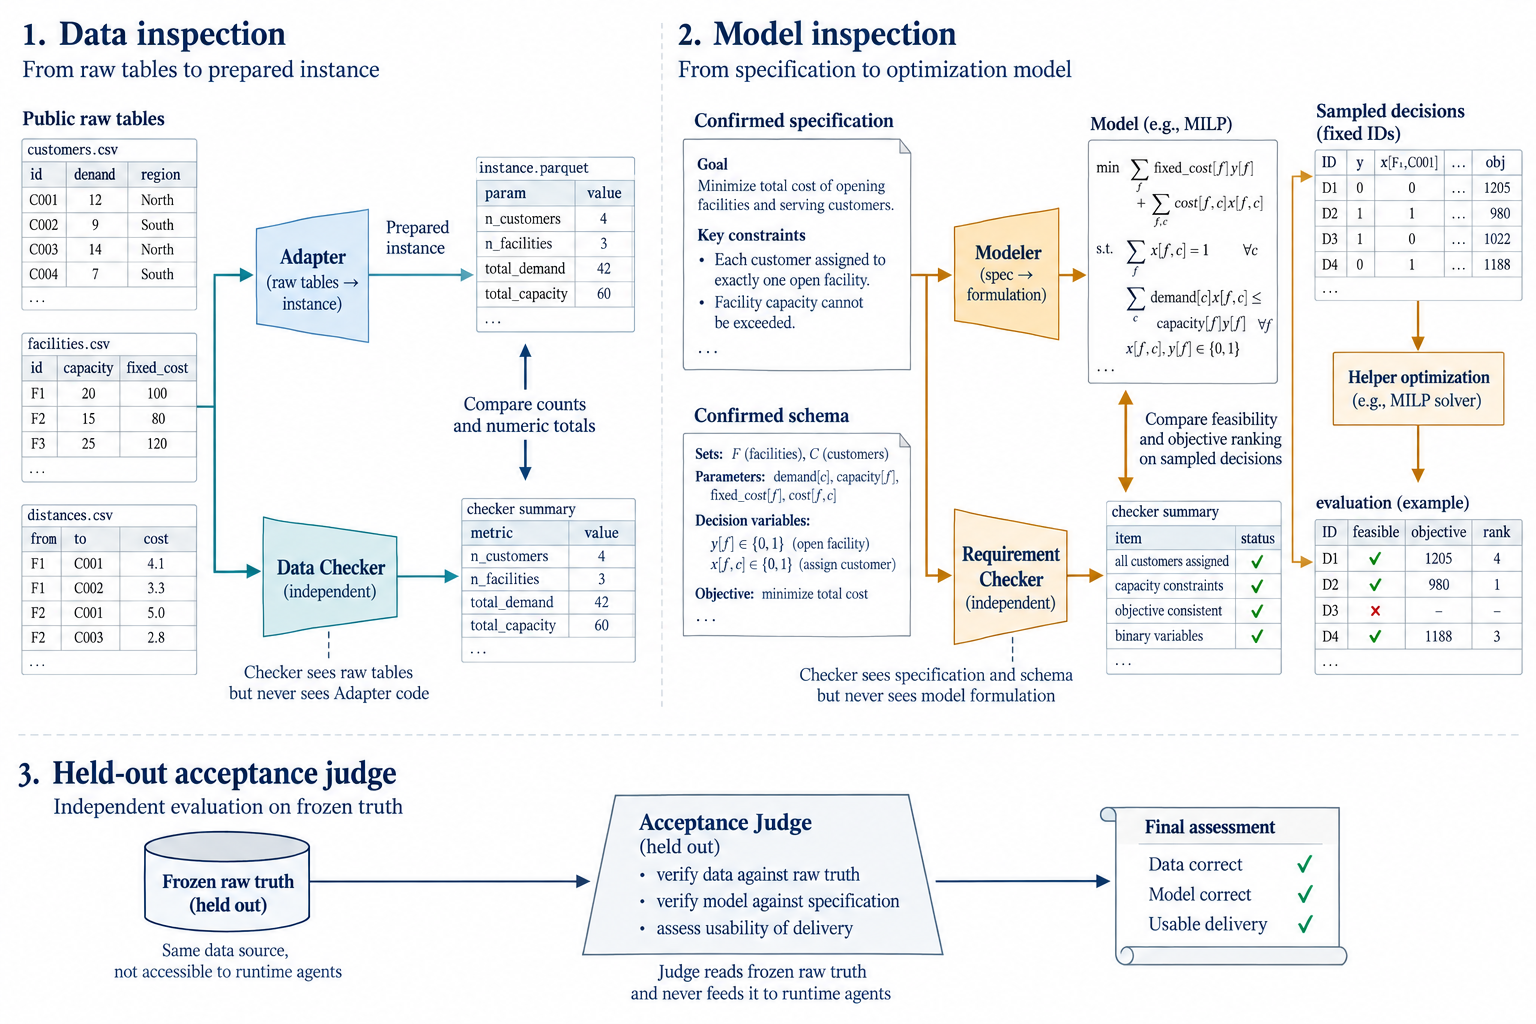
\includegraphics[width=\textwidth]{figures/verification-illustrated.png}
\caption{Illustrative data inspection, requirement inspection and external acceptance judging. Tables,
formulations, evaluation values and check marks are schematic examples, not experimental results.
Agents receive bounded raw-table profiles and write code that operates on full tables; the Requirement
Checker does not see the formulation. Helper optimization is used where supported. Checker agreement is
evidence rather than a correctness guarantee; held-out judge truth is not supplied to runtime agents.}
\label{fig:verificationlayers}
\end{figure*}


\subsection{Compilation, solving and recovery}
Equalities use squared penalties; inequalities use binary or unary slack, or approximate unbalanced
penalization\cite{montanez2024unbalanced}. Exclusion and implication constraints use pairwise penalties.
PyQUBO placeholders allow weights to change without recompiling the same encoding\cite{pyquboDocs}.
Explicit labels preserve decision and auxiliary indices. Encoded penalty diagnostics supplement original
constraint checks; incorrectly populated slack can give a penalty even for a feasible original decision.

The backend interface supports simulated annealing (SA), Compal GPU Annealer (CGA), Fujitsu Digital Annealer
(DA)\cite{aramon2019digital}, and D-Wave direct QPU or Leap Hybrid BQM. The experiments use SA, CGA and Leap
Hybrid. No direct-QPU experiment is reported; DA was blocked by an account usage limit.
The default policy is selected initially. Explicit alternatives include LLM tuning, rules, random search,
Optuna\cite{akiba2019optuna} and penalty-only searches. Bounds, parameter ranges and encoding-specific checks
reject invalid proposals. A single-flip penalty floor is a heuristic, not a proof of global-optimum preservation.
For large models, agents receive constraint families rather than every individual constraint.

Before annealing, a time-limited HiGHS preflight checks feasibility. Proven infeasibility avoids a solver call;
timeout remains unknown. A feasible conventional solution supplies a comparison baseline. For quadratic
objectives, bounded local improvement does not certify an optimum. If annealing has no feasible result or
trails a validated baseline beyond the configured tolerance, that baseline may be delivered with its source stated.

Evidence routes repairs to data preparation or modelling instead of treating every failure as a weak penalty.
An acquisition schema mismatch can trigger a new model and renewed preparation. Download failures do not
by themselves justify changing a model. Requirement-check disagreements can supply model-repair evidence.
Repairs are bounded, validated before activation and share the remaining solver budget. Comparisons on original
data protect existing formulas and fixed settings; changed requirements or unresolved substitutions need user
confirmation. These checks cannot prove that a repair preserves natural-language meaning.

Model code, data and provenance are versioned together. Generated code runs in separate processes with
timeouts, providing process isolation rather than a security sandbox. Supported penalty searches resume from
recorded histories, while changed-model or unresolved-call checkpoints are rejected. Saved solutions survive
visualization or explanation failures.

\subsection{Optional modelling-pattern retrieval}
The Modeler can select up to three general patterns by title from a local library and receive their text as
additional context. Repairs retain the selected IDs. This bounded retrieval supplies building blocks, not a
case-specific completed formulation. Its modelling-stage effect is distinct from retrieval of tuning knowledge;
no positive end-to-end retrieval effect is assumed.
